\chapter{Under the Hood}

\cvmfs\ has a modular structure and relies on several open source libraries.
Figure~\ref{fig:cvmfsblocks} shows the internal building blocks of \cvmfs.
Most of those libraries are shipped with the \cvmfs\ tarball and can be linked statically to keep the system dependencies minimal.

\begin{figure}
	\begin{center}
		%\documentclass[a4paper, 11pt]{article}

%\usepackage{tikz,ifthen}
%\usetikzlibrary{shapes,matrix,shadows,fit,backgrounds}

%\begin{document}
\begin{tikzpicture}
\edef\blockwidth{7em} 
\edef\blockheight{2.5em}
\scope[ 
      block/.style={
         anchor=south west,
         rectangle,
         very thick,
         drop shadow,
         rounded corners=3mm,
         minimum width=\blockwidth,
         minimum height=\blockheight},   
      buildingblock/.style={
         block,
         draw=red!50!black!50,
         top color=white,
         bottom color=red!50!black!20},
      module/.style={
         block,
         draw=green!50!black!50,
         top color=white,
         bottom color=green!50!black!20},
      fuse/.style={
         block,
         draw=blue!50!black!50,
         top color=white,
         bottom color=blue!50!black!20},
      blocklabel/.style={
         anchor=north west,
         inner ysep=-0.5ex,
         font=\large\sf},
      every fit/.style={
         rectangle,
         very thick,
         draw=gray},
      font={\small\sf}
   ]
   
   \edef\spacesep{2ex}
   \edef\numofelemsperline{3}

   % Bulding Blocks
   \edef\numofelems{8} 
   \pgfmathparse{floor(\numofelems/\numofelemsperline)*\numofelemsperline}\edef\fitsuntil{\pgfmathresult}
   \foreach \i / \name in {0 / SHA1, 1 / MD5, 2 / zlib, 3 / SQLite, 4 / libcurl, 5 / libcrypto, 6 / Fuse, 7 / redirfs}
   {
      \ifthenelse{\i<\fitsuntil}{\edef\offset{0}}{
         \pgfmathparse{((\numofelemsperline-mod(\numofelems,\numofelemsperline))/2)*(\blockwidth+\spacesep)}\edef\offset{\pgfmathresult}}
      \pgfmathparse{\offset + mod(\i,\numofelemsperline)*(\blockwidth+\spacesep)}\edef\blockx{\pgfmathresult}
      \pgfmathparse{floor(\i/\numofelemsperline) * (\blockheight+\spacesep)}\edef\blocky{\pgfmathresult}
      \coordinate (blockxy) at (\blockx pt, \blocky pt);
      \node [buildingblock] at (blockxy) {\name};
   }
   \pgfmathparse{\numofelemsperline*(\blockwidth+\spacesep)-\spacesep}\edef\extremx{\pgfmathresult}
   \pgfmathparse{ceil(\numofelems/\numofelemsperline)*(\blockheight+\spacesep)-\spacesep + 4ex}\edef\extremy{\pgfmathresult}
   \coordinate (extremxy) at (\extremx pt, \extremy pt);
   \node (bb bottom left) at (0,0) {};
   \node (bb top right) at (extremxy) {};
   \begin{pgfonlayer}{background}
      \node [fit=(bb bottom left) (bb top right),top color=red!50!black!20,bottom color=white] (bb box) {};
      \node [blocklabel] at (0,\extremy pt) {Building Blocks};
   \end{pgfonlayer}
   

   % Modules
   \pgfmathparse{\extremy+2*\spacesep}\edef\yoffset{\pgfmathresult}
   \edef\numofelems{5}
   \pgfmathparse{floor(\numofelems/\numofelemsperline)*\numofelemsperline}\edef\fitsuntil{\pgfmathresult}
   \foreach \i / \name in {0 / Catalog, 1 / Cache, 2 / {Quota / LRU}, 3 / Trace Capturing, 4 / {VFS Filter}}
   {
      \ifthenelse{\i<\fitsuntil}{\edef\offset{0}}{
         \pgfmathparse{((\numofelemsperline-mod(\numofelems,\numofelemsperline))/2)*(\blockwidth+\spacesep)}\edef\offset{\pgfmathresult}}
      \pgfmathparse{\offset + mod(\i,\numofelemsperline)*(\blockwidth+\spacesep)}\edef\blockx{\pgfmathresult}
      \pgfmathparse{\yoffset + floor(\i/\numofelemsperline) * (\blockheight+\spacesep)}\edef\blocky{\pgfmathresult}
      \coordinate (blockxy) at (\blockx pt, \blocky pt);
      \node [module] at (blockxy) {\name};
   }
   \pgfmathparse{\numofelemsperline*(\blockwidth+\spacesep)-\spacesep}\edef\extremx{\pgfmathresult}
   \pgfmathparse{\yoffset+ceil(\numofelems/\numofelemsperline)*(\blockheight+\spacesep)-\spacesep + 4ex}\edef\extremy{\pgfmathresult}
   \coordinate (extremxy) at (\extremx pt, \extremy pt);
   \node (mod bottom left) at (0,\yoffset pt) {};
   \node (mod top right) at (extremxy) {};
   \begin{pgfonlayer}{background}
      \node [fit=(mod bottom left) (mod top right),top color=green!50!black!20,bottom color=white] (mod box) {};
      \node [blocklabel] at (0,\extremy pt) {Components};
   \end{pgfonlayer}
   
   %fuse
   \pgfmathparse{\extremy+2*\spacesep}\edef\yoffset{\pgfmathresult}
   \edef\numofelems{2}
   \pgfmathparse{floor(\numofelems/\numofelemsperline)*\numofelemsperline}\edef\fitsuntil{\pgfmathresult}
   \foreach \i / \name in {0 / \cvmfs, 1 / cvmfs\_sync}
   {
      \ifthenelse{\i<\fitsuntil}{\edef\offset{0}}{
         \pgfmathparse{((\numofelemsperline-mod(\numofelems,\numofelemsperline))/2)*(\blockwidth+\spacesep)}\edef\offset{\pgfmathresult}}
      \pgfmathparse{\offset + mod(\i,\numofelemsperline)*(\blockwidth+\spacesep)}\edef\blockx{\pgfmathresult}
      \pgfmathparse{\yoffset + floor(\i/\numofelemsperline) * (\blockheight+\spacesep)}\edef\blocky{\pgfmathresult}
      \coordinate (blockxy) at (\blockx pt, \blocky pt);
      \node [fuse] at (blockxy) {\name};
   }
   \pgfmathparse{\numofelemsperline*(\blockwidth+\spacesep)-\spacesep}\edef\extremx{\pgfmathresult}
   \pgfmathparse{\yoffset+ceil(\numofelems/\numofelemsperline)*(\blockheight+\spacesep)-\spacesep + 4ex}\edef\extremy{\pgfmathresult}
   \coordinate (extremxy) at (\extremx pt, \extremy pt);
   \node (fuse bottom left) at (0,\yoffset pt) {};
   \node (fuse top right) at (extremxy) {};
   \begin{pgfonlayer}{background}
      \node [fit=(fuse bottom left) (fuse top right),top color=blue!50!black!20,bottom color=white] (fuse box) {};
      \node [blocklabel] at (0,\extremy pt) {User Interface};
   \end{pgfonlayer}      
\endscope
\end{tikzpicture}
%\end{document}

	\end{center}
	\caption{\cvmfs\ block diagram.}
	\label{fig:cvmfsblocks}
\end{figure}


\section{File Catalog}

A \cvmfs\ repository is defined by its \indexed{file catalog}\index{catalog|see{file catalog}}.
The file catalog is an \product{SQLite} database~\cite{sqlite} having a single table that lists files and directories together with its \indexed{metadata}.
The table layout is shown in Table~\ref{tab:catalog}.

\begin{table}
	\begin{center}
		\begin{tabular}[b]{ccc}
			\begin{tabular}{l|l}
				\bf Field & \bf Type \\\hline
				\bf Path MD5 & 128\,Bit Integer \\
				Parent Path MD5 & 128\,Bit Integer \\
				inode & Integer \\
				SHA1 Content Hash & 160\,Bit Integer \\
				Size & Integer \\
				Mode & Integer \\
				Last Modified & Timestamp \\
				Flags & Integer \\
				Name & String \\
				Symlink & String \\
			\end{tabular} &
			\qquad & 
			\begin{tabular}{l|l}
				\bf Flags & \bf Meaning\\\hline
				1 & Directory \\
				2 & Transition point to a nested catalog \\
				33 & Root directory of a nested catalog \\
				3 & Regular file \\
				4 & Symbolic link
			\end{tabular}
		\end{tabular}
	\end{center}
	\caption{Metadata information stored per directory entry.}
	\label{tab:catalog}
\end{table}

In order to save space we do not store absolute paths.
Instead we store \indexed{MD5} hash values of the absolute path names.
Symlinks\index{symbolic link} are kept in the catalog.
Symlinks may contain \indexed{environment variable}s that will be dynamically resolved by \cvmfs\ on access.
The \indexed{SHA1} content hash referrs to the \indexed{zlib}-compressed version of the file.
Flags indicate the type of an directory entry (see Table~\ref{tab:catalog}).

A file catalog contains a \index{time to live} (TTL), stored in seconds.
The catalog TTL advises clients to check for a new version of the catalog, when expired.
Checking for a new catalog version takes place with the first file system operation on a \cvmfs\ volume after the TTL has expired.
The default TTL is one hour.
If a new catalog is available, \cvmfs\ delays it's loading for the period of the \cvmfs\ kernel cache life time (default: 1 minute).
During this drain-out period, the kernel caching is turned off.
The first file system operation on a \cvmfs\ volume after that additional delay will apply a new file catalog and kernel caching is turned back on.

\subsection{Nested Catalogs}
In order to keep catalog sizes reasonable\footnote{As a rule of thumb, file catalogs up to 25\,MB (compressed) are reasonably small.}, repository subtrees may be cut and stored as separate \newterm{\indexed{nested catalog}s}.
There is no limit on the level of nesting.
A reasonable approach is to store separate software versions as separate nested catalogs.
Figure~\ref{fig:nested} shows the directory structure which we use for the ATLAS repository.
\begin{figure}
	\begin{center}
		\framebox{%\documentclass[a4paper, 11pt]{article}

%\include{jtex}
%\usepackage{tikz,ifthen}
%\usetikzlibrary{arrows,positioning,shapes,topaths,calc,fit,backgrounds,matrix,shadows}

%\begin{document}

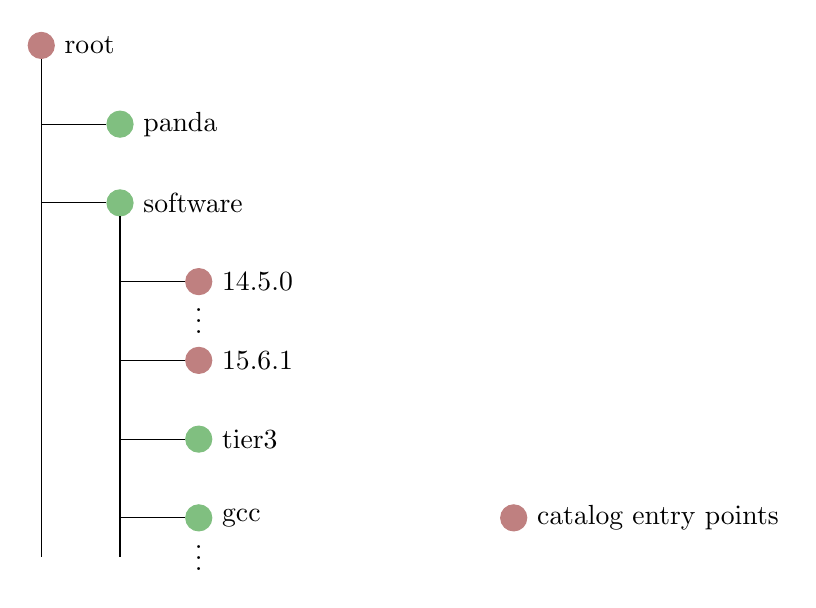
\begin{tikzpicture}
	[
		dirent/.style={
			circle,
			draw=green!50!black!50,
			fill=green!50!black!50
		}
	]
	\node[dirent,label=right:root,red!50!black!50,fill=red!50!black!50] (root) at (0,0) {};
	\node[dirent,label=right:panda] (panda) at (1, -1) {};
	\node[dirent,label=right:software] (software) at (1, -2) {};
	\node[dirent,label=right:14.5.0,red!50!black!50,fill=red!50!black!50] (1450) at (2, -3) {};
	\node[] (dots1) at (2, -3.4) {$\vdots$};
	\node[dirent,label=right:15.6.1,red!50!black!50,fill=red!50!black!50] (1561) at (2, -4) {};
	\node[dirent,label=right:tier3] (tier3) at (2, -5) {};
	\node[dirent,label=right:gcc] (gcc) at (2, -6) {};
	\node[] (dots2) at (2, -6.4) {$\vdots$};
	\node[dirent,label=right:catalog entry points,red!50!black!50,fill=red!50!black!50] (key) at (6,-6) {};
	
	%\node[dirent] (d2) at (0.4, 0.8) {};
	%\node[dirent,red!50!black!50,fill=red!50!black!50] (d21) at (0.8, 0.4) {};
	%\node[dirent] (d22) at (0.8, 0) {};
	%\node[scale=0.175] (file) at (2, 0.8) {\pdfimage{file.pdf}};
	
	\draw (root) -- (0,-1) -- (panda);
	\draw (0,-1) -- (0,-2) -- (software);
	\draw (0,-2) -- (0,-6.5);
	\draw (software) -- (1,-3) -- (1450);
	\draw (1,-3) -- (1,-4) -- (1561);
	\draw (1,-4) -- (1,-5) -- (tier3);
	\draw (1,-5) -- (1,-6) -- (gcc);
	\draw (1,-6) -- (1,-6.5);
\end{tikzpicture}
%\end{document}}
	\end{center}
	\caption{Directory structure useds for the ATLAS repository.}
	\label{fig:nested}
\end{figure}

When a subtree is moved into a nested catalog, its entry directory serves as \indexed{transition point} for nested catalogs.
This directory appears as empty directory in the parent catalog with Flags set to 2.
The same path appears as root-directory in the nested catalog with Flags set to 33.
Because the \indexed{MD5} hash values refer to full absolute paths, nested catalogs store the root \indexed{path prefix}\index{prefix|see{path prefix}}.
This prefix is prepended transparently by \cvmfs.
The SHA-1 key of nested catalogs is stored in the parent catalog.
Therefore, the root catalog fully defines an entire repository.

Loading of nested catalogs happens on demand by \cvmfs\ on the first attempt to access of anything inside, \ie a user won't see the difference between a single large catalog and several nested catalogs.
While this usually avoids unnecessary catalogs to be loaded, recursive operations like \texttt{find} can easily bypass this optimization.
Nested catalogs are also separate \indexed{mount point}s.
This allows for mounting \cvmfs\ deep\index{deep mount} into a repository, for instance one might mount a specific software release.
Note that in this case the \lstinline{deep_mount} mount option has to be set accordingly.


\subsection{$\mu$-Catalogs}
The $\mu$-catalogs can be constructed in addition to the normal file catalogs.
The $\mu$-catalogs can be considered as a special case of nested catalogs, in which each directory is a nested catalog.
Essentially they are a precalculated \texttt{ls -la} for all directories.
They are implemented as SQlite catalogs as well having the same structure as normal catalogs.
The SHA-1 content hashes of the $\mu$-catalogs are stored in the hash field of the directory entries in the catalog table.


\subsection{Catalog Signature}\index{signature}
In order to provide authoritative information about a repository \indexed{publisher}, file catalogs may be signed by an \indexed{X.509} \indexed{certificate}.
It is important to note that it is sufficient to sign just the file catalog.
Since every file is listed with its SHA1 content hash inside the catalog, we gain a secure chain and may speak of a ``signed repository''.

The signature is created using the \texttt{cvmfs\_sign} utility.
The \texttt{cvmfs\_sign} utility takes a X.509 certificate together with its private key in order to sign a catalog and its nested catalogs.
On the client side, \cvmfs\ supports a \newterm{\indexed{trusted mode}} in which only validly signed catalogs are mounted.

In order to validate file catalog signatures, \cvmfs\ uses a \indexed{white-list} procedure.
The white-list contains the SHA1 fingerprints of known publisher certificates and a timestamp.
A white-list is valid for 30 days.
It is signed by a private RSA key, which we refer to as \cernvm\ \newterm{master key}.
The master key is kept offline on a secure smart card at \cern.
So the security of the master key is ensured by 2-factor authentication (possession of the smart card and knowledge of the pin).
The smart card is used with a smart card reader with pin pad.
Neither the key nor the pin are ever exposed outside the scope of those secure devices.
The public RSA key that corresponds to the master key is distributed with the \cvmfs\ sources and the \cvmfs\ rpm as well as with every instance of \cernvm.

In addition, \cvmfs\ checks certificate fingerprints against a local blacklist (default location is \texttt{/etc/cvmfs/blacklist}).
The blacklisted fingerprints have to be in the same format than the fingerprints on the white-list.
The blacklist has precedence over the white-list.

As crypto engine, \cvmfs\ use \product{libcrypto} from the \product{OpenSSL} project~\cite{openssl}.
Figure~\ref{fig:security} shows the trust chain with a signed repository.
\begin{figure}
	\begin{center}
		%\documentclass[a4paper, 11pt]{article}\usepackage{tikz,ifthen}\usetikzlibrary{arrows,positioning,shapes,topaths,calc,fit,backgrounds,matrix,shadows}\begin{document}

\begin{tikzpicture}
	[block/.style={node distance=1cm,rounded corners,draw,minimum height=0.7cm,minimum width=3cm},
	 fig/.style={}]
	
	\node[fig,gray] (release manager) at (6cm,0cm) {\parbox{2cm}{\centering release\\
\includegraphics[width=1.25cm]{figures/releasemanager}\\manager}};
	\node[fig,gray,anchor=north] (whitelist) at (0cm,-2cm) {\parbox{3cm}{\centering \parbox[top][2cm][c]{2.5cm}{
\includegraphics[width=2.5cm]{figures/cernvm}}\\certificate white-list}};
	\node[fig,gray,anchor=north] (web server) at (12cm,-2cm) {\parbox{3cm}{\centering \parbox[top][2cm][c]{2.5cm}{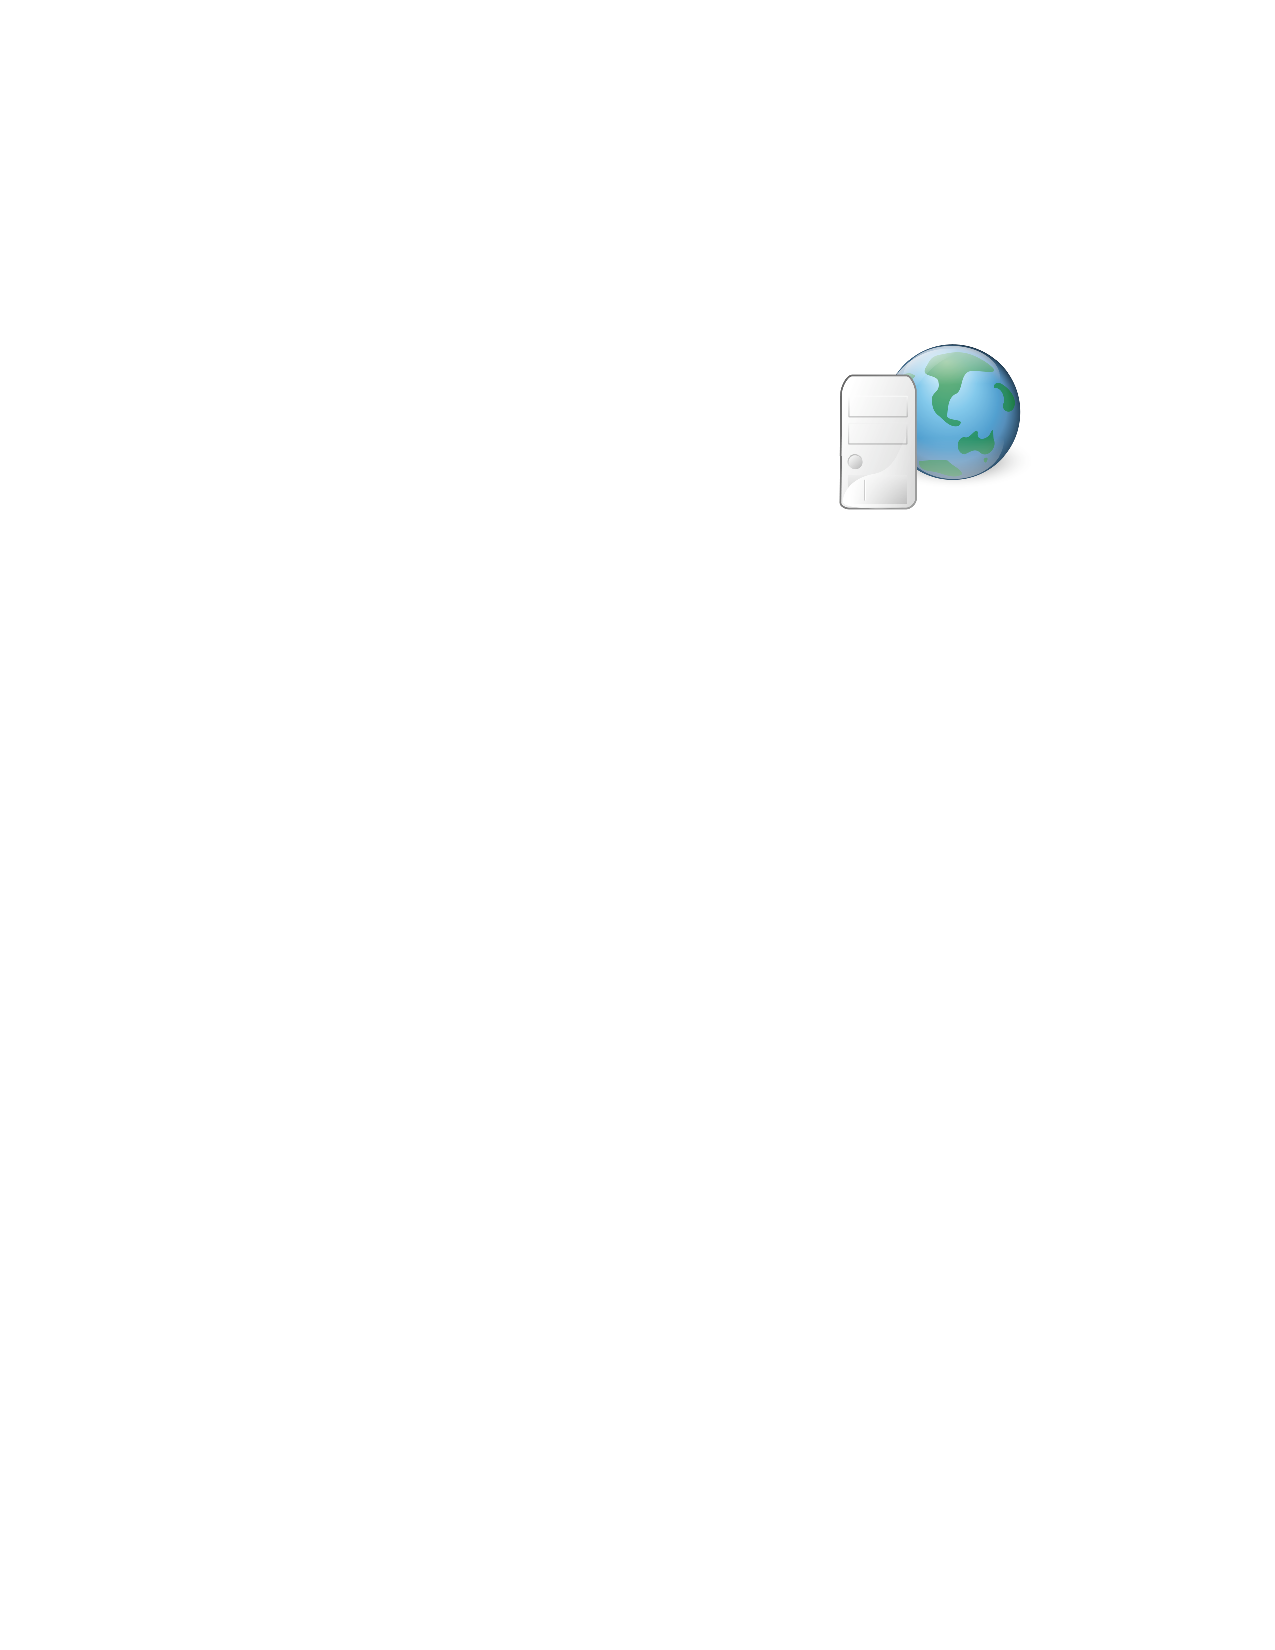
\includegraphics[width=1.75cm]{figures/webserver}}\\repository}};
	\node[block,green!50!black,very thick] (cvmfs) at (6cm,-9cm) {\parbox{3.5cm}{\centering{\scshape CernVM-FS +\\CernVM} public key}};
	
	\draw[->,gray,very thick] (release manager.west) -- node[gray,fill=white] {\parbox{2cm}{\centering
\includegraphics[width=1cm]{figures/fingerprint}\\ fingerprint}} (whitelist.north);
	\draw[->,gray,very thick] (release manager.east) -- node[gray,fill=white] {\parbox{2cm}{\centering
\includegraphics[width=1cm]{figures/sign-cert}\\ sign repository}} (web server.north);
	\draw[->,gray,very thick] (whitelist.east) -- node[white,fill] {\parbox{2cm}{\centering
\includegraphics[width=1cm]{figures/sign}\\ \textcolor{gray}{sign whitelist}}} ($(whitelist.east) + (8.75,0)$);
	
	\draw[->,very thick,blue!75,curve to,out=200,in=90] (web server.south west) to node[blue!75,fill=white] {\parbox{3cm}{\centering {\tikz \node[fill,draw,circle,inner sep=1pt]{\textcolor{white}1};}\\download\\signed catalog +\\signed whitelist}} (cvmfs.north);
	\node[blue!75,above left=of cvmfs,xshift=0.75cm,yshift=-0.75cm] {\parbox{3cm}{\centering {\tikz \node[fill,draw,circle,inner sep=1pt]{\textcolor{white}2};}\\verify whitelist +\\check fingerprint}};
	\draw[->,very thick,blue!75,curve to,out=270,in=45] (web server.south) to node[blue!75,below] {\parbox{2cm}{\centering {\tikz \node[fill,draw,circle,inner sep=1pt]{\textcolor{white}3};}\\download\\files}} (cvmfs.north east);
	\node[blue!75] at (6cm,-10.5cm) {\parbox{4cm}{\centering {\tikz \node[fill,draw,circle,inner sep=1pt]{\textcolor{white}4};}\\compare secure hash\\against catalog entry}};
\end{tikzpicture} 

%\end{document}

	\end{center}
	\caption{Trust chain with a signed repository.}
	\label{fig:security}
\end{figure}


%\section{Repository Layout}
%\label{sct:repository}

\section{Exploited HTTP Features}
The particular way of using the \indexed{HTTP} protocol has significant impact on the performance and usability of \cvmfs.
The benefit from extended HTTP/1.1 features like \indexed{keep-alive}, \indexed{cache-control}\index{no-cache|see{cache-control}} and \indexed{pipelining}~\cite{rfc2616} requires the intermediate \indexed{proxy server}s and \indexed{web server}s to support them, too.
In any way, \cvmfs\ has to work using just plain old HTTP/1.0~\cite{rfc1945}.
Internally, \cvmfs\ uses the \product{libcurl} library~\cite{libcurl}.

The HTTP behaviour affects a ``\indexed{cold cache}d'' \cvmfs\ system.
As soon as all necessary files are cached, there is only network traffic when a catalog TTL\index{time to live} expires.
Usually we'll see network traffic right after booting a \cernvm\ for the first time, after switching to another experiment environment, and after a new software version has been published.

Downloading files is serialized by \cvmfs.
This avoids wasting the network channel by parallel downloads of the same file.

\subsection{Forward Proxies}
\label{sct:proxies}
\cvmfs\ has a dedicated HTTP \indexed{proxy configuration}, independent from system-wide settings.
We encourage sites to setup a proxy that mirrors the \cvmfs\ repository, in order to decrease latency and increase reliability.
Instead of a single proxy, \cvmfs\ uses a \newterm{\indexed{chain of load-balanced proxy groups}}.
If a proxy fails, \cvmfs\ automatically switches to the next group in the chain (\newterm{automatic fail-over}).
The chain is internally treated as ring buffer, \ie after probing the last proxy in the chain, the first proxy is probed again.
To avoid endless loops, for each file download the number of switches is restricted by the total number of proxies.
Each of the proxy groups is itself a list of proxy servers from which one of the servers is selected randomly.
This leads to a \newterm{load-balancing} of proxy servers.
Within a load-balanced group, fail-over takes place to another random server of that group until all proxy servers in the group failed in a row.

The chain of proxy groups is specified by a string of semicolon separated entries, each group is a list of pipe separated hostnames\footnote{The usual proxy notation rules apply, like \texttt{http://proxy1:8080|http://proxy2:8080;DIRECT}}.
The \texttt{DIRECT} keyword for a hostname avoids using proxies.
%\cvmfs\ ships with a script that orders a set of proxies according to the \indexed{round trip time}\index{RTT|see{round trip time}} for a download.

\subsection{Timeouts}
\cvmfs\ does an effort to recover from broken network links.
There is a configurable timeout for connection attempts and for very slow downloads (mount option \lstinline{-o timeout}), which is 10 seconds by default.
A download is considered to be ``very slow'' if the transfer rate is below 100 Bytes/second for more than the timeout interval.
A very slow download is treated like a broken connection.
However, stalled DNS requests may still make the \cvmfs\ process look hanging.
Therefore, we recommend a local DNS caching server, such as a BIND caching server or \texttt{nscd}.

On timeout, \cvmfs\ switches to the next proxy server and/or host if defined.
Otherwise it returns with an EIO error to the application.
\cvmfs\ distinguishes between a proxied connection and a direct connetion and allows different timouts for the two cases.

\cvmfs\ uses exponential backoff for download failures.
That prevents request storms to web servers from applications trying to open a file in an endless loop.
The backoff is triggered by consequtive download errors within 10 seconds.

\subsection{Keep-Alive}\index{keep-alive}
Although the HTTP protocol overhead is small in terms of data volume, in high latency networks we suffer from the bare number of requests: Each request-response cycle has a penalty of at least the network round trip time. 
Using plain HTTP/1.0, this results in at least 3x(\indexed{round trip time}) additional running time per file download for TCP handshake, HTTP GET, and TCP connection finalisation.
By including the \texttt{Connection:~Keep-Alive} header into HTTP requests, we advise the HTTP server end to keep the underlying TCP connection opened.
This way, overhead ideally drops to just round trip time for a single HTTP GET.
The impact of the keep-alive feature is shown in Figure~\ref{fig:keepalive}.
\begin{figure}
	\begin{center}
		\resizebox{0.5\linewidth}{!}{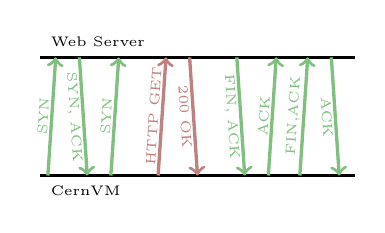
\begin{tikzpicture}
	[
		legend/.style={
			font=\tiny,
			outer sep=-2pt
		},
		legendframe/.style={
			font=\tiny
		},
		seq/.style={
			->, 
			very thick, 
			green!50!black!50	
		},
		http/.style={
			->, 
			very thick, 
			red!50!black!50	
		}
	]
	
	\draw[very thick]  (0,1.5) -- node[legendframe,above,anchor=south west] {Web Server} (0,1.5) -- (4,1.5);
	\draw[very thick]  (0,0) -- node[legendframe,below,anchor=north west] {CernVM} (0,0) -- (4,0);
	
	\draw[seq] (0.1,0) -- node[legend,sloped,above] {SYN} (0.2,1.5);
	\draw[seq] (0.5,1.5) -- node[legend,sloped,below] {SYN, ACK} (0.6,0);
	\draw[seq] (0.9,0) -- node[legend,sloped,above] {SYN} (1,1.5);
	
	\draw[http] (1.5,0) -- node[legend,sloped,above] {HTTP GET} (1.6,1.5);
	\draw[http] (1.9,1.5) -- node[legend,sloped,below] {200 OK} (2,0);
	
	\draw[seq] (2.5,1.5) -- node[legend,sloped,below] {FIN, ACK} (2.6,0);
	\draw[seq] (2.9,0) -- node[legend,sloped,above] {ACK} (3,1.5);
	\draw[seq] (3.3,0) -- node[legend,sloped,above] {FIN,ACK} (3.4,1.5);
	\draw[seq] (3.7,1.5) -- node[legend,sloped,below] {ACK} (3.8,0);
	
\end{tikzpicture}}
	\end{center}
	\caption{Impact of keep-alive header on multiple file downloads.}
	\label{fig:keepalive}
\end{figure}

This feature, of course, somewhat sabotages a server-side \indexed{load balancing}.
However, exploiting the HTTP keep-alive feature does not affect scalability per se. 
The servers and proxies may safely close idle connections anytime, in particular if they run out of resources.
In practice, the maximum connection duration has to be set carefully for the HTTP deamon.

\subsection{Cache Control}\index{cache-control}
\label{sct:cachecontrol}
In a limited way, \cvmfs\ advises intermediate web caches how to handle its requests.
Therefor it uses the \texttt{Pragma:~no-cache} and the \texttt{Cache-Control:~no-cache} headers in certain cases.
These cache control headers apply to both, \indexed{forward proxies} as well as \indexed{reverse proxies}.
However, this is by no means a guarantee that intermediate proxies fetch a fresh original copy (though they should).

By including these headers, \cvmfs\ tries to not fetch outdated cache copies.
This has to be handled with care, of course, in order to not overload\index{load balancing} the repository source server.
In case \cvmfs\ downloads a corrupted file from a proxy server, it retries having the HTTP \texttt{no-cache} header set.
This way, the corrupted file gets replaced in the proxy server by a fresh copy from the backend.

\subsection{Identification Header}
\cvmfs\ sends a custom header (\lstinline{X-CMFS2}) to be identified by the web server.
In \cernvm\ we use this header to rewrite URL's to the respective repository format for \cvmfs\ version 1 or \cvmfs\ version 2.
If you have set the \cernvm\ GUID, this GUID is also transmitted.

\section{Disk Cache}

The \indexed{disk cache} stores files with a name according to their \indexed{SHA-1} content hash.
Thereby the disk cache is decoupled from any specific directory hierarchy.
Identical files stored in different directories are stored only once.

Each running \cvmfs\ instance has a separate \indexed{cache directory}. 
The local cache directory (directories \texttt{00}, \dots, \texttt{ff}) can be accessed in parallel to a running \cvmfs, \ie files can be deleted for instance anytime\footnote{While the design supports it, we however strongly suggest not to tamper with the cache directory because it will make the local LRU database inconsistent.}. 
During the download, files reside in the \texttt{txn} directory. 
At the very latest point they are renamed into their content addressable SHA1 names atomically by \texttt{rename()}. 

\subsection{Managed Disk Cache}\index{managed disk cache}
\label{sct:mamangedcache}
The traditional \cvmfs\ disk cache just grows until the system runs out of disk space.
Files may be deleted manually from the cache directories, but this is a cumbersome job.

By using a \newterm{managed disk cache}, \cvmfs\ maintains cache size restrictions and replaces files according to the \indexed{least recently used}\index{LRU|see{least recently used}} (LRU) strategy~\cite{lru06}.
In order to keep track of files sizes and relative file access times, \cvmfs\ sets up another \product{SQLite} database in the cache directory, the \newterm{\indexed{cache catalog}}.
The cache catalog contains a single table; its structure is shown in Table~\ref{tab:cachecatalog}.
\begin{table}
	\begin{center}
		\begin{tabular}{l|l}
			\bf Field & \bf Type \\\hline
			\bf SHA1 & 160\,Bit Integer \\
			Size & Integer \\
			Access Sequence & Integer \\
			Pinned & Integer \\
			File type (chunk or file catalog) & Integer
		\end{tabular}
	\end{center}
	\caption{Cache catalog table structure.}
	\label{tab:cachecatalog}
\end{table}

Note that \cvmfs\ does not enforce a certain cache size.
Instead \cvmfs\ works with two customizable \indexed{soft limit}s, the \newterm{cache quota} and the \newterm{cache threshold}.
When exceeding the cache quota, files are deleted until the overall cache size is less than or equal to the cache theshold.
The cache quota is for data files as well as file catalogs.
Currently loaded catalogs are pinned in the cache, \ie they will not be deleted.
On unmount, pinned file catalogs are updated with the highest sequence number.

The cache catalog can be constructed from scratch on mount.
Re-constructing the cache catalog is necessary when the managed cache is used for the first time and every time when ``unmanaged'' changes occurred to the cache directory.
This happens, for instance, if \cvmfs\ is mounted with the managed cache feature turned off.
Re-construction has to be triggered manually.

For performance reasons, the cache management runs as a separate thread.
This thread takes care of updating access times and deleting of files when necessary.
The \cvmfs\ \texttt{open} function talks via \indexed{pipe}s to that thread.
A typical compilation benchmark on \cvmfs\ shows 1\%-2\% additional \indexed{running time} caused by the managed cache.


\section{File System Traces}\index{traces}\index{file system traces|see{traces}}
\cvmfs\ has an optional file system operations tracer.
The tracer creates logs of usage, which can---for instance---be used as profiling information for pre-fetching.
The trace file is created in \indexed{CSV} format (see Figure~\ref{fig:traces}).
\begin{figure}
	\centering
	\begin{verbatim}
"1481074921.015","1","/root/i686-pc-linux-gnu/include/TQObject.h","OPEN"
"1481074931.030","1","/root/i686-pc-linux-gnu/include/KeySymbols.h","OPEN"
"1481074931.220","3","/root/i686-pc-linux-gnu/include/KeySymbols.h","READ (TRY)"
"1481074964.565","3","/root/i686-pc-linux-gnu/include/KeySymbols.h","READ 7407@0"
"1481074965.005","1","/root/i686-pc-linux-gnu/include/TRootCanvas.h","OPEN"
	\end{verbatim}
	\caption{Example snippet of a trace log. The first columns stores time stamps as number of microseconds starting from the Unix epoch. The second column stores the event type. Negative event types are reserved for \cvmfs\ internal events.}
	\label{fig:traces}
\end{figure}

The tracing runs in a separate thread and adapts the \emph{tread-safe trace buffer}, a technique used for multi-thread debugging~\cite[Chapter 8]{multicore06}.
Since traces are kept in a memory ring buffer\footnote{Usually, each trace record requires two atomic \texttt{fetch-and-add} operations.} and written to disk in blocks of thousands of lines, the performance overhead for tracing is almost negligible; for our application benchmarks it is below measurement error.\index{running time}

%\section{Pre-fetching}\index{pre-fetching}
%\label{sct:prefetching}

\section{System Interface}
\label{sct:interface}

Since \cvmfs\ is a read-only file system, there are only few non-trivial call-back functions to implement.
These \indexed{call-back function}s provide the system interface.

\subsection{{\tt \indexed{mount}} / {\tt \indexed{re-mount}}}
On mount, the file catalog has to be loaded.
First, the file catalog \indexed{checksum} \texttt{.cvmfspublished} is loaded.
If \cvmfs\ runs in \indexed{trusted mode} or if it finds a signature in the checksum, the catalog is only accepted on successful validation of the \indexed{signature}.
In order to validate the signature, the certificate and the \indexed{white-list} are downloaded in addition if not found in cache.
If the download failes for whatever reason, \cvmfs\ tries to load a local file catalog copy.
As long as all requested files are in the disk cache as well, \cvmfs\ continues to operate even without network access (\newterm{\indexed{offline mode}}).

If there is no local copy of the catalog checksum or the downloaded checksum and the cache copy differ, \cvmfs\ downloads a fresh copy of the file catalog.
If the checksum matches the file catalog, the cache copies are replaced by the downloaded versions and the new catalog is mounted.
Otherwise, the procedure is repeated avoiding intermediate proxy servers (see Section~\ref{sct:cachecontrol}).

\subsection{\tt stat}
Requests for file attributes are entirely served from the mounted catalog\index{file catalog}, \ie there is no network traffic involved.
This function is called as pre-requisite to other file system operations and therefore the most frequently called FUSE callback.
In order to minimize relatively expensive \product{SQLite} queries, \cvmfs\ uses a 2-way associative / direct-mapped negative and positive hybrid cache, having the first bits of the \indexed{MD5} path name hash as key.
The size of the cache is determined according to compilation benchmarks monitored with \product{Valgrind}~\cite{callgrind} and according to LHCb application benchmarks.

Additionally, this callback takes care of the catalog TTL.\index{time to live}
If the TTL is expired, the catalog is re-mounted on the fly.
Note that a re-mount might possibly break running programs.
We rely on careful repository publishers that produce more or less immutable directory trees, \ie new repository versions just add files.

If a directory with a \indexed{nested catalog} is accessed for the first time, the respective catalog is mounted in addition to the already mounted catalogs.
Loading nested catalogs is transparent to the user.

\subsection{\tt readlink}
A symlink\index{symbolic link} is served from the file catalog.
As a special extension, \cvmfs\ detects \indexed{environment variable}s in symlink strings written as \texttt{\$(VARIABLE)}.
Those variables are expanded by \cvmfs\ dynamically on access (in the context of the cvmfs process).
This way, a single symlink can point to different locations depending on the environment.
This is helpful, for instance, to dynamically select software package versions residing in different directories.

\subsection{\tt readdir}
A directory listing is served by an SQL query on the file catalog.
Though the ``parent''-column is indexed (\cf Table~\ref{tab:catalog}), this is a relatively slow function.
We expect directory listing to happen rather seldom.

\subsection{\tt open / read}
The \texttt{open()} call has to provide Fuse with a \indexed{file handle} for a given path name.
In \cvmfs\ file requests are always served from the \indexed{disk cache}.
The Fuse file handle is a file descriptor valid in the context of the \cvmfs\ process.
It points into the disk cache directory.
Read requests are translated into the \texttt{pread()} system call.

Opening a path name is done in the following steps:
\begin{enumerate}
	\item The path name is hashed with \indexed{MD5}
	\item Using this MD5 hash, the file catalog is asked for the \indexed{SHA1} key for the given path name
	\item If the file is not in the disk cache, it is downloaded from the \indexed{repository}
\end{enumerate}

\subsection{\tt getxattr}
\cvmfs\ uses extended attributes to display additional repository information.
Currently there are two supported attributes:
\begin{description}
	\item[hash]
		Shows the SHA-1 hash of a regular file as listed in the file catalog.
		For a directory, shows the SHA-1 hash of the $\mu$-catalog, if available.
	\item[lhash]
		Shows the SHA-1 hash of a regular file as stored in the local cache, if available.
	\item[revision]
		Shows the file catalog revision of the mounted root catalog, an auto-increment counter increased on every synchronization of shadow tree and repository.
		The value is the same for all directories, symbolic links and regular files of the mount point.
	\item[pid]
		Shows the \cvmfs\ process id.
	\item[version]
		Shows the version of the loaded \cvmfs\ binary.
	\item[expires]
		Shows the remaining life time of the hosting (nested) file catalog in minutes.
	\item[maxfd]
		Shows the maximum number of file descriptors available to file system clients.
	\item[usedfd]
		Shows the number of file descriptors currently issued to file system clients.		
	\item[nioerr]
		Shows the total number of I/O errors encoutered since mounting.			
	\item[proxy]
		Shows the currently active HTTP proxy.
	\item[host]
		Shows the currently active HTTP replica server.
	\item[uptime]
		Shows the time passed since mounting in minutes.
	\item[nclg]
		Shows the number of currently loaded nested catalogs.
	\item[nopen]
		Shows the overall number of \texttt{open()} calls since mounting.
	\item[ndwonload]
		Shows the overall number of downloaded files since mounting.
	\item[timeout]
		Shows the timeout for proxied connections in seconds.
	\item[timeout\_direct]
		Shows the timeout for direct connections in seconds.
	\item[rx]
		Shows the overall amount of downloaded kilobytes.
	\item[speed]
		Shows the average download speed.
\end{description}

Extended attributes can be queried using the \texttt{attr} command.
For instance, \texttt{attr -g hash /cvmfs/atlas.cern.ch/ChangeLog} returns the SHA-1 key of the file at hand.
The extended attributes are used by the \texttt{cvmfs\_config stat} command in order to show a current overview of health and performance numbers.

\subsection{Dynamic Configuration}
\label{sct:dynconf}

\cvmfs\ is capable of communicating to the user at runtime.
Thereby certain parameters can be configured and changed while the file system is mounted.
To do so, \cvmfs\ sets up a temporary \indexed{socket} in the \indexed{cache directory}, \texttt{cvmfs\_io}.
Communication is based on a simple command-response scheme.
The enclosed \texttt{cvmfs-talk} script takes care of writing to and reading from the socket.
Currently \cvmfs\ handles the following commands:
\begin{description}
	\item[\tt flush] Flushes the entries in the trace buffer from memory to disk.\index{traces}
	\item[\tt cache size] Returns the combined size of the data files and file catalogs in the (managed) disk cache.\index{managed disk cache}\index{disk cache}
	\item[\tt cache list] Returns the list of downloaded files that reside in the (managed) disk cache.\index{managed disk cache}\index{disk cache}
	\item[\tt cache list catalog] Returns the list of downloaded file catalogs that reside in the (managed) disk cache.\index{managed disk cache}\index{disk cache}
	\item[\tt cache list pinned] Returns the list of pinned (loaded) file catalogs that reside in the (managed) disk cache.\index{managed disk cache}\index{disk cache}
	\item[\tt cleanup <MB>] Unlinks files from the (managed) disk cache until cache size is less than or equal to the specified size in MB.
	\item[\tt clear file <path>] Removes <path> from local cache.
	\item[\tt mountpoint] Gets the mount point.
	\item[\tt remount] Checks for a new root file catalog.
	\item[\tt revision] Gets the currently mounted repository revision.
	\item[\tt max ttl info] Gets the maximum file catalog TTL.
	\item[\tt max ttl set <minutes>] Sets the maximum file catalog TTL.
	\item[\tt host info] Gets the host chain and their RTT, if already probed.
	\item[\tt host probe] Orders the host chain according to round trip time.  This happens automatically every 1000 downloads.
	\item[\tt host switch] Switches to the next host in the chain.
	\item[\tt host set <host chain>] Sets a new host chain.
	\item[\tt proxy info] Gets the currently active proxy server.
	\item[\tt proxy rebalance] Randomly selects a new proxy server from the current load-balancing group.
	\item[\tt proxy group switch] Switches to the next load-balance proxy group in the chain.
	\item[\tt proxy set <proxy list>] Sets a new chain of load-balance proxy groups.
	\item[\tt timeout info] Gets the network timeouts with and without proxy.
	\item[\tt timeout set <proxy> <direct>] Sets the network timeouts in seconds.
	\item[\tt reset error counters] Resets the internal counter for failed I/O operations.
	\item[\tt pid] Returns the process id of the \texttt{cvmfs2} main process (not the watchdog).
	\item[\tt version] Returns the version number of the running \cvmfs\ instance.
	\item[\tt version patchlevel] Returns the version patchlevel of the running \cvmfs\ instance.
	\item[\tt open catalogs] Returns mount point, last modified timestamp, and expiry date of currently loaded catalogs.  These are not necessarily all cached catalogs.
\end{description}

The \texttt{cvmfs-talk} command is also used by the cvmfs service in order to reload the configuration.
Reloadable are all parameters with a ``set'' variant.

\section{Repository Synchronization}

Repositories are not immutable, every now and then they get updated. 
This might be installation of a new release or a patch for an existing release.  
But, of course, each time only a small portion of the repository is touched, say 2\,GB out of 100\,GB.
In order to not process an entire shadow tree on each synchronization, we use a file system change log as basis of the synchronization.
To this end, we use a \cvmfs\ \newterm{filter} for \redirfs~\cite{redirfs05} (cf.~Fig.~\ref{fig:cvmfsflt}).
The \cvmfs\ filter intercepts VFS system calls that might change file data or file meta data on a given directory sub-tree.
We refer to such VFS calls as \newterm{writing calls}.

\begin{figure}
	\begin{center}
		%\documentclass[a4paper, 11pt]{article}\usepackage{tikz,ifthen}\usetikzlibrary{arrows,positioning,shapes,topaths,calc,fit,backgrounds,matrix,shadows}\begin{document}\begin{tikzpicture}
\begin{tikzpicture}
	\tikzset{
		hiddenblock/.style={node distance=0.75cm,minimum height=0.7cm,font=\footnotesize},
		block/.style={hiddenblock,minimum width=2cm,draw},
		wideblock/.style={block,minimum width=3.5cm},
		thinblock/.style={node distance=0.5cm,font=\footnotesize,draw,minimum width=2cm},
			background/.style={
			rectangle,
			fill=gray!10,
			inner sep=0.2cm,
			rounded corners=1mm},
		cvmfsfltarrow/.style={green!75!black,->,very thick},
		action/.style={->}
	}
	
	\node[block] (p1) at (0,0) {process 1};
	\node[hiddenblock,right=of p1] (p dots) {$\cdots$};
	\node[block, right=of p dots] (pn) {process $n$};
	
	\node[node distance=0.8cm] (splitleft) [below=of p1,xshift=-2.75cm] {};
	\node[node distance=0.8cm] (splitright) [below=of pn,xshift=6cm] {};
	\draw[dashed,blue] (splitleft) -- node[blue,above,at start,anchor=south west] {\footnotesize user space} node[blue,below,at start,anchor=north west] {\footnotesize kernel space} (splitright);
	
	\node[wideblock,yshift=-2.4cm] (vfs) [below of=p dots] {\parbox{3cm}{\centering VFS\\inode cache\\dentry cache}};
	\node[block] (nfsd) [left=of vfs] {nfsd};
	\node[wideblock] (redirfs) [below=of vfs] {\bf redirfs};
	\node[hiddenblock] (fs dots) [below=of redirfs] {$\cdots$};
	\node[block] (ext3) [left=of fs dots] {Ext3};
	\node[block] (nfs) [right=of fs dots] {NFS};
	
	\node[block,green!50!black,anchor=east,fill=white,xshift=-1cm] (chardev) at (splitright) {\texttt{/dev/cvmfs}};
	
	% filters
	\begin{scope}[xshift=6cm,yshift=-2.7825cm]
		\node[thinblock,gray] (filter 1) {filter 1};
		\node[thinblock,green!50!black,yshift=-0.25cm] (cvmfsflt) [below=of filter 1] {cvmfsflt};
		\node[thinblock,gray,yshift=-0.25cm] (filter m) [below=of cvmfsflt] {filter $m$};
		\path (filter 1) -- node[gray,midway,yshift=0.1cm] {\footnotesize $\vdots$} (cvmfsflt);
		\path (cvmfsflt) -- node[gray,midway,yshift=0.1cm] {\footnotesize $\vdots$} (filter m);
		\begin{pgfonlayer}{background}
	        		\node[background, fit=(filter 1) (filter m)] {};
		\end{pgfonlayer}
	\end{scope}
	
	% ring buffer
	\begin{scope}[line width=3mm,rotate=90,scale=0.4,yshift=-22cm,xshift=-10cm]
		\node[text centered,text width=1cm]{\footnotesize call buffer};
		\draw[thin,gray] (0,0) circle (2.2cm) circle (1.4cm);
		\draw[green!75!black] (0:1.8cm) arc (0:-231:1.8cm);
		\draw[green] (-231:1.8cm) arc (-231:-245:1.8cm);
		\node (newline) at (122:2.2cm) {};
		\node (firstline) at (-7:2.2cm) {};

		\newcount\mycount
		\foreach \angle in {0,144,...,3599}
		{
      			\mycount=\angle\relax
			\divide\mycount by 10\relax
			\draw[black!15,thick] (\the\mycount:14mm) -- (\the\mycount:22mm);
    		}
	\end{scope}
	
	\draw[action] (p1) -- node[fill=white,yshift=0.75ex] {\footnotesize syscall} (vfs);
	\draw[action] (pn) -- node[fill=white,yshift=0.75ex] {\footnotesize syscall} (vfs);
	\draw[action] (nfsd) -- (vfs);
	\draw[action] (vfs) -- (redirfs);
	\draw[action] (redirfs.north east) -- (filter 1.west);
	\draw[action] (filter m.west) -- (redirfs.south east);
	\draw[action] (redirfs) -- (ext3);
	\draw[action] (redirfs) -- (nfs);
	
	\draw[cvmfsfltarrow,curve to,out=0,in=225] (cvmfsflt) to (newline.center);
	\draw[cvmfsfltarrow,curve to,out=90,in=270] (firstline.center) to (chardev.south);
	
	\node[block,green!50!black] (sync) at (pn -| chardev) {\texttt{cvmfs\_sync}};
	\draw[green!50!black,very thick,->] (chardev.north) -- (sync.south);
\end{tikzpicture}
%\end{tikzpicture}\end{document}

	\end{center}
	\caption{\cvmfs\ filter for \redirfs: Writing VFS calls are captured and written to a character device to create a file system change log.}
	\label{fig:cvmfsflt}
\end{figure}

\cvmfs\ ships with two kernel modules, \texttt{redirfs} and \texttt{cvmfsflt}.
These modules have to be loaded in this order.
Once loaded, they are configured via {\scshape sysfs}~\cite{sysfs05}.
See Table~\ref{tab:sysfs} for a list of control files.

The \cvmfs\ VFS filter has three modes of operation:
\begin{description}
	\item[Normal Operation] Capture writing VFS calls to the call buffer, whose tail is connected to a character device.
	\item[Call Buffer Full] Block writing VFS calls. If the \texttt{O\_NONBLOCK} flag is set, do not block but return \texttt{EAGAIN}.
	\item[Synchronizing Repository] Forbid writing VFS calls (return \texttt{EPERM}).
\end{description}

\begin{table}
	\begin{center}
		\begin{tabularx}{\linewidth}{llX}
			\bf File & \bf Permission & \bf Purpose \\\hline
			\texttt{lockdown} & r/w & Forbid writing VFS calls (during synchronization) \\
			\texttt{noll} & r & Number of remaining entries in the VFS call buffer \\
			\texttt{nowops} & r & Number of remaining writing VFS calls \\
		\end{tabularx}
	\end{center}
	\caption{Sysfs control files for \texttt{cvmfsflt} in \texttt{/sys/fs/redirfs/filters/cvmfsflt}.}
	\label{tab:sysfs}
\end{table}

In order to set up file system capturing, one can use the following commands:
\begin{lstlisting}[language=bash]
modprobe redirfs
modprobe cvmfsflt
if [ ! -c /dev/cvmfs ]; then
  major=`grep cvmfs /proc/devices | awk '{print $1}'`
  mknod /dev/cvmfs c $major 0
fi
echo -n "a:i:$MY_FILTER_PATH" > /sys/fs/redirfs/filters/cvmfsflt/paths
\end{lstlisting}
The data stream of the character device has to be stored into a log file for further processing with \texttt{cvmfs\_sync}.
If the character device is not read, the call buffer will eventually become full and writing VFS calls to the filtered path are blocked by the \cvmfs\ filter.

The following steps have to be done before starting a synchronization run:
\begin{enumerate}
	\item Lock the filtered path down using the {\scshape sysfs} control file (cf.~Table~\ref{tab:sysfs})
	\item Wait for the remaining writing VFS call counter to become zero
	\item Wait for the remaining call entry buffer counter to become zero
\end{enumerate}

In order to unload, one can use the following commands:
\begin{lstlisting}[language=bash]
echo -n "c\0" > /sys/fs/redirfs/filters/cvmfsflt/paths
echo -n "1\0" > /sys/fs/redirfs/filters/cvmfsflt/unregister
rmmod cvmfsflt
\end{lstlisting}
